\section{数学建模和计算}
\subsection{改进DH参数表}
改进DH参数表(Modified DH,MDH)是一种用于描述机器人机械臂各个关节之间的几何关系的方法。MDH参数表比传统的DH参数表更灵活,可以处理更多类型的机器人结构。基于我们小组的机械臂模型参数,设计MDH如表\ref{tab:4}所示:

\begin{table}[h]
	\centering
    \caption{ABB-IRB-1200模型MDH参数表}
    \label{tab:4}
    \vspace{5pt}
	\setlength{\tabcolsep}{4mm}{
	\begin{tabular}{
	>{\columncolor[HTML]{DAE8FC}}c |
	>{\columncolor[HTML]{DAE8FC}}c |
	>{\columncolor[HTML]{DAE8FC}}c |
	>{\columncolor[HTML]{DAE8FC}}c |
	>{\columncolor[HTML]{DAE8FC}}c |
	>{\columncolor[HTML]{DAE8FC}}c |
	>{\columncolor[HTML]{DAE8FC}}c }
	\hline\hline
	\diagbox{Parameter}{Joints}		 & 1           & 2           & 3             & 4            & 5            & 6            \\ \hline
	$\theta$ & $\theta_1+0$ & $\theta_2+0$ & $\theta_3-90$ & $\theta_4+0$ & $\theta_5+0$ & $\theta_6+0$ \\ \hline
	$d$      & 0.38         & 0           & 0             & 0.34          & 0            & 0.27          \\ \hline
	$\alpha_{i-1}$ & 0           & -90          & 0             & -90          & 90           & -90           \\ \hline
	$a_{i-1}$      & 0           & 0           & 0.35          & 0            & 0            & 0            \\ \hline\hline
	\end{tabular}}
\end{table}

MDH参数表的确定,对后续雅各比矩阵计算、运动学和动力学的计算和仿真等工作都有重要意义。

\subsection{Jacobi矩阵}
机器人雅克比矩阵描述的是关节速度和末端笛卡尔速度和角速度之间的关系。计算雅各比矩阵的常用方法有矢量积法和微分变换法,其中使用矢量积法得到的雅各比矩阵是相对于基坐标系的,微分变换法得到的是相对于末端坐标系的。由于相对于基坐标系的雅各比矩阵比较直接,我们采用矢量积法来求解。

我们所设计的机器人六个关节均为转动关节。而对于转动关节,雅各比矩阵各列元素可以用以下公式表示:

\begin{equation}
    \begin{bmatrix}
        v\\
        w
    \end{bmatrix}=\begin{bmatrix}
        z_i \times ^ip_n^0\\
        z_i
    \end{bmatrix} \dot{q}_i; \quad  J_i =\begin{bmatrix}
        z_i \times ^ip_n^0\\
        z_i
    \end{bmatrix}
\end{equation}

列向量$J_i$表示末端速度、角速度与i关节的角速度之间的关系,将6个列向量组合即可得到机器人的雅各比矩阵,即:
\begin{equation}
    J=\begin{bmatrix}
        J_1 & J_2 & J_3 & J_4 & J_5 & J_6
    \end{bmatrix}
\end{equation}

具体来说,使用矢量积法得到雅各比矩阵需要经过以下步骤,首先根据MDH参数表得到各连杆间的变换矩阵${^{i-1}T}_i$,之后计算各连杆至基坐标系的变换矩阵${^0T}_i$,然后从得到的矩阵中,可以找到$z_i$和$^ip_n^0$的对应元素,最后使用矢量积法公式就可以得到雅各比矩阵了。

根据所设计的机器人的MDH参数表,我们可以利用以下公式计算各连杆间的变换矩阵${^{i-1}T}_i$:
\begin{equation}
    {^{i-1}T}_i=\begin{bmatrix}
        cos \theta_i & -sin \theta_i & 0 & a_{i-1}\\
        sin \theta_i cos \alpha_{i-1} & cos \theta_i cos \alpha_{i-1} & -sin \alpha_{i-1} & -sin \alpha_{i-1}d_i\\
        sin \theta_i sin \alpha_{i-1} & cos \theta_i sin \alpha_{i-1} & cos \alpha_{i-1} & cos \alpha_{i-1}d_i\\
        0 & 0 & 0 & 1
    \end{bmatrix}
\end{equation}

带入各关节的参数,可以得到:
\begin{equation*}
    ^0T_1=\left[ \begin{matrix}	cos\!\:\theta _1&		-sin\!\:\theta _1&		0&		0\\	sin\!\:\theta _1&		cos\!\:\theta _1&		0&		0\\	0&		0&		1&		0.38\\	0&		0&		0&		1\\\end{matrix} \right] \mathrm{      }^1T_2=\left[ \begin{matrix}	cos\!\:\theta _2&		-sin\!\:\theta _2&		0&		0\\	0&		0&		1&		0\\	-sin\!\:\theta _2&		-cos\!\:\theta _2&		0&		0\\	0&		0&		0&		1\\\end{matrix} \right] 
\end{equation*}

\begin{equation*}
    ^2T_3=\left[ \begin{matrix}	sin\!\:\theta _3&		cos\!\:\theta _3&		0&		0.35\\	-cos\!\:\theta _3&		sin\!\:\theta _3&		0&		0\\	0&		0&		1&		0\\	0&		0&		0&		1\\\end{matrix} \right] \mathrm{      }^3T_4=\left[ \begin{matrix}	cos\!\:\theta _4&		-sin\!\:\theta _4&		0&		0\\	0&		0&		1&		0.34\\	-sin\!\:\theta _4&		-cos\!\:\theta _4&		0&		0\\	0&		0&		0&		1\\\end{matrix} \right] 
\end{equation*}

\begin{equation*}
    ^4T_5=\left[ \begin{matrix}	\cos \!\:\theta _5&		-\sin \!\:\theta _5&		0&		0\\	0&		0&		-1&		0\\	\sin \!\:\theta _5&		\cos \!\:\theta _5&		0&		0\\	0&		0&		0&		1\\\end{matrix} \right] \mathrm{      }^5T_6=\left[ \begin{matrix}	cos\!\:\theta _6&		-sin\!\:\theta _6&		0&		0\\	0&		0&		1&		0.27\\	-sin\!\:\theta _6&		-cos\!\:\theta _6&		0&		0\\	0&		0&		0&		1\\\end{matrix} \right] 
\end{equation*}

之后,我们可以计算出各连杆至基坐标系的变换矩阵${^0T}_i$,并从中得到$z_i$和$^ip_n^0$的对应元素,最后使用矢量积法公式就可以得到雅各比矩阵了。

\begin{equation}
    \left\{
        \begin{aligned}
            ^0T_2&=^0T_1 \times ^1T_2\\
            ^0T_3&=^0T_1 \times ^1T_2 \times ^2T_3\\
            ^0T_4&=^0T_1 \times ^1T_2 \times ^2T_3 \times ^3T_4\\
            ^0T_5&=^0T_1 \times ^1T_2 \times ^2T_3 \times ^3T_4 \times ^4T_5\\
            ^0T_6&=^0T_1 \times ^1T_2 \times ^2T_3 \times ^3T_4 \times ^4T_5 \times ^5T_6
        \end{aligned}
    \right.
\end{equation}

$z_i$为3维列向量,其3个元素即为${^0T}_i$第三列的前三个元素。$^ip_n^0$为3维列向量,$^ip_n^0=^6p_0-^ip_0$,其中$^ip_0 $($i$取值范围为1-6)也是3维向量,其3个元素即为${^0T}_i$第四列的前三个元素。

将$z_i$和$^ip_n^0$对应带入矢量积法的公式中,最终可以得到雅各比矩阵。若取初始情况,即$\theta_i=0$($\theta_3$有初始$-90^\circ$的偏置角),结果为:

\begin{equation*}
    J=\begin{bmatrix}
        0 & 0 & 0 & 0 & 0 & 0\\
        0.96 & 0 & 0 & 0 & 0 & 0\\
        0 & -0.96 & -0.61 & 0 & -0.27 & 0\\
        0 & 0 & 0 & 1 & 0 & 1\\
        0 & 1 & 1 & 0 & 1 & 0\\
        1 & 0 & 0 & 0 & 0 & 0
    \end{bmatrix}
\end{equation*}

上述过程可以通过MATLAB代码实现,首先设计计算各连杆间的变换矩阵${^{i-1}T}_i$的函数:

\textbf{Code 1 {\quad} 计算各连杆间的变换矩阵${^{i-1}T}_i$的函数}
\begin{lstlisting}
function T = trans(theta, d, a, alpha)
T = [cos(theta),-sin(theta),0,a;
sin(theta)*cos(alpha), cos(alpha)*cos(theta),-sin(alpha),-d*sin(alpha);
sin(theta)*sin(alpha), sin(alpha)*cos(theta), cos(alpha), d*cos(alpha);
0, 0, 0, 1];
end

\end{lstlisting}

然后将MDH参数带入,求得$^{i-1}T_i$,这里以计算$^5T_6$为例:
\begin{lstlisting}
T56 = trans(theta6, 0.27, 0, -pi/2);   %连杆6至连杆5的变换矩阵
\end{lstlisting}

接着使用矩阵连乘的方法得到各连杆至基坐标系的变换矩阵$^0T_i$,以求$^0T_6$为例:
\begin{lstlisting}
T06 = T01*T12*T23*T34*T45*T56;   %连杆6至基坐标系的变换矩阵
\end{lstlisting}

然后从$^0T_i$中得到$z_i$和$^ip_n^0$的对应元素,带入矢量积法公式中得到$J_i$,以求$J_1$为例:
\begin{lstlisting}
P01 = [T01(1,4);T01(2,4);T01(3,4)];
P06 = [T06(1,4);T06(2,4);T06(3,4)];
z1 = T01(1:3,3);
j1 = [cross(z1,P06-P01);z1];   %矢量积法求J1
\end{lstlisting}

最后,将6个列向量组合得到机器人的雅各比矩阵:
\begin{lstlisting}
Jacobian1 = [j1,j2,j3,j4,j5,j6];   %机器人的雅各比矩阵
\end{lstlisting}

在MATLAB的robotics toolbox库中有求解雅各比矩阵的对应函数,其中jacob0代表相对于基坐标系的雅各比矩阵求解,与我们使用矢量积法得到的结果相同。以下是初始状态下两种方法得到的结果对比,如下图\ref{fig:13}所示:

\begin{figure}[h]
    \centering
    \subfigure[工具包函数jacob0的计算]{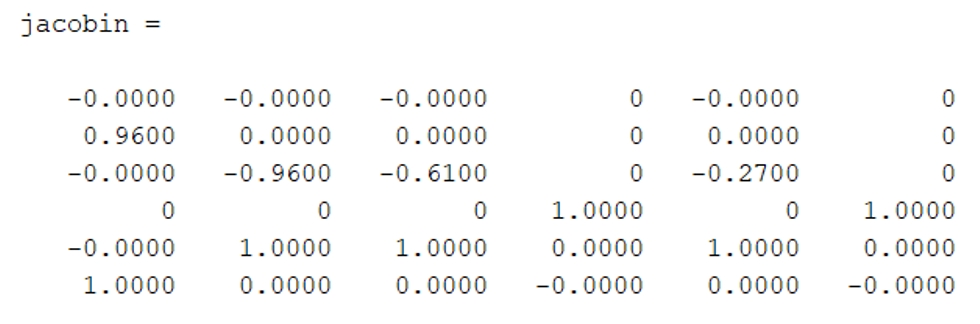
\includegraphics[width=0.4\textwidth]{Image/fig20.jpg}}
    \subfigure[使用矢量积法的雅各比矩阵]{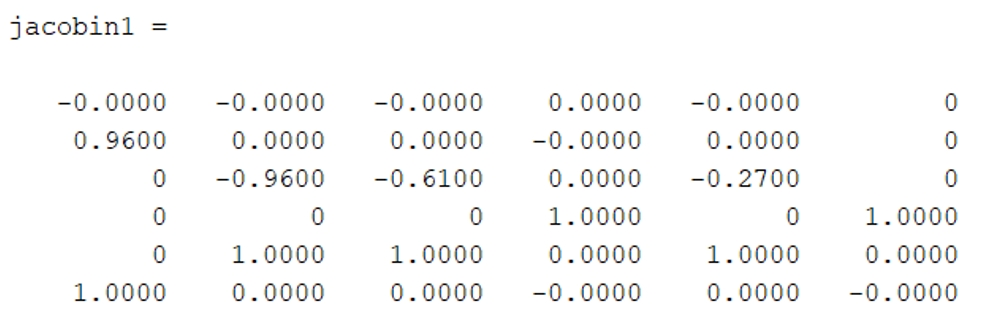
\includegraphics[width=0.4\textwidth]{Image/fig21.jpg}}
    \caption{两种方法得到的雅各比矩阵对比}
    \label{fig:13}
\end{figure}

\subsection{安装方式和自重比计算}
在机械臂设计与应用中,自重负载比是一个关键的参数,它直接影响到机械臂的稳定性和工作效率。在本次研究中,我们考察了不同安装方式对机械臂自重负载比的影响,包括地面安装、墙壁安装与悬挂安装。

首先需要计算各安装方式的最大载荷:我们通过调研和计算,得出了每种安装方式所能承受的最大力。
\begin{enumerate}
    \item \textbf{地面安装}:地面安装方式下,机械臂的自重负载比相对较低,因为地面提供了最大的支撑力。
    \item \textbf{墙壁安装}:机械臂的自重负载比最高。因为墙壁提供的支撑力需要同时承受机械臂自重和操作时的动载荷。
    \item \textbf{悬挂安装}:自重负载比介于地面安装和墙壁安装之间。悬挂安装需要考虑更多的动态因素,如机械臂的摆动和扭矩。
\end{enumerate}

根据上述数据,我们可以计算出各种安装方式的最大载荷,如表\ref{tab:5}所示:

\begin{table}[h]
    \centering
    \caption{不同安装方式的最大载荷}
    \vspace{5pt}
    \label{tab:5}
    \begin{tabular}{
    >{\columncolor[HTML]{ECF4FF}}c 
    >{\columncolor[HTML]{ECF4FF}}c 
    >{\columncolor[HTML]{ECF4FF}}c 
    >{\columncolor[HTML]{ECF4FF}}c }
    \hline \hline
    安装方式   & 力        & 最大载荷(N) & 总最大载荷(N) \\ \hline
    Ground & $F_{xy}$ & 1620    & 2284     \\ \hline
    Ground & $F_z$    & 1610    & /        \\ \hline
    Wall   & $F_{xy}$ & 1940    & 2358     \\ \hline
    Wall   & $F_z$    & 1340    & /        \\ \hline
    Hang   & $F_{xy}$ & 1620    & 2284     \\ \hline
    Hang   & $F_z$    & 1610    & /        \\ \hline \hline
    \end{tabular}
    \end{table}

接下来我们进行了力的示意与分析工作:我们使用了力的示意图来分析不同安装方式下机械臂受力的情况。图\ref{fig:14}与图\ref{fig:15}展示了机械臂在不同安装方式下的受力方向和力的分布情况。

\begin{figure}[htbp]
    \centering
    \subfigure[受力前视图]{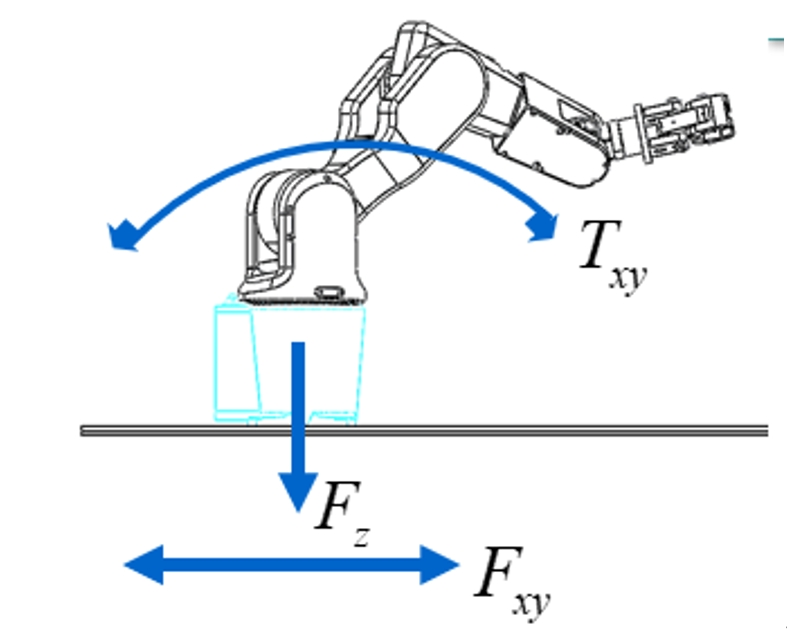
\includegraphics[width=0.4\textwidth]{Image/fig23.jpg}
    \label{fig:14}}
    \subfigure[受力上视图]{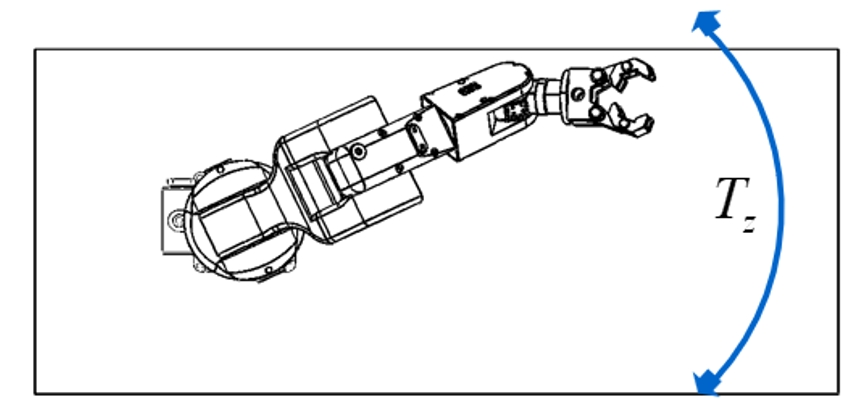
\includegraphics[width=0.4\textwidth]{Image/fig24.jpg}
    \label{fig:15}}
    \caption{机械臂受力示意图}
\end{figure}

最终我们得到最大自重负载比:

在机械臂自重52kg的条件下,我们得出最大自重负载比出现在墙壁安装方式下,最大自重负载比为:
\begin{equation*}
    \frac{2358}{52 \times 9.8}=4.53
\end{equation*}

该值表明在墙壁安装情况下,机械臂能够承受的最大载荷为其自重的4.53倍。墙壁安装方式能够在保持稳定性的前提下,承受较大的操作载荷。

我们对上述过程进行了分析,得出以下结论:
\begin{itemize}
    \item 装方式对自重负载比的影响显著:墙壁安装方式虽然提供了最高的自重负载比,但需要在设计时充分考虑安装结构的强度和稳定性。
    \item 优化设计的重要性:为了在实际应用中实现最佳性能,需要根据具体的使用环境和操作要求,选择合适的安装方式,并对机械臂的设计进行优化。
\end{itemize}


\section{运动学计算和实现}
\subsection{正向运动学}
正向运动学描述了从机器人关节空间到末端执行器位置和姿态的变换。具体来说,正向运动学计算的是给定关节变量(如关节角度或关节位移)时,末端执行器在工作空间中的位置和方向。

根据MDH参数表,我们在5.2小节已经计算得到了各连杆间的变换矩阵,我们据此可以计算得到末端位姿:
$$
    ^0T_6=^0T_1 \times ^1T_2 \times ^2T_3 \times ^3T_4 \times ^4T_5 \times ^5T_6=
$$
\begin{figure}[htbp]
    \centering
    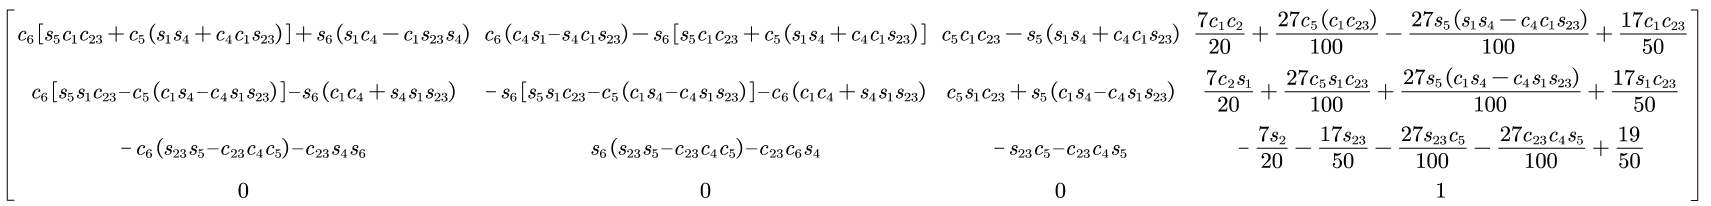
\includegraphics[width=\textwidth]{Image/fig25.jpg}
\end{figure}

其中$s_i=sin\theta_i,c_i=cos\theta_i,s_{ij}=sin\left(\theta_i+\theta_j\right),c_{ij}=cos\left(\theta_i+\theta_j\right)$。

即实现了正向运动学——根据各关节角度信息计算得到末端位姿信息.

\subsection{逆向运动学}
机器人的逆运动学共有8组解,以下为求解过程。

设$\boldsymbol{p}_w$为4坐标系原点在基坐标系的坐标。

设输入矩阵为:
\begin{equation}
    T_{6}^{0}=\left[ \begin{matrix}	R_{6}^{0}&		p_{6}^{0}\\	0&		1\\\end{matrix} \right] 
\end{equation}

通过末端位姿反推到
\begin{equation}
    p_w=p_{6}^{0}-R_{6}^{0}\left[ \begin{array}{c}	0\\	0\\	0.27\\\end{array} \right] =\left[ \begin{array}{c}	p_{wx}\\	p_{wy}\\	p_{wz}\\\end{array} \right] 
\end{equation}

正向运算:
\begin{equation}
    T_{3}^{0}=\left[ \begin{matrix}	c_1s_{23}&		c_1c_{23}&		-s_1&		\frac{7c_1c_2}{20}\\	s_1s_{23}&		s_1c_{23}&		c_1&		\frac{7s_1c_2}{20}\\	c_{23}&		-s_{23}&		0&		\frac{19}{50}-\frac{7s_2}{20}\\	0&		0&		0&		1\\\end{matrix} \right]
\end{equation}

\begin{equation}
    \left[ \begin{array}{c}	p_{wx}\\	p_{wy}\\	p_{wz}\\	1\\\end{array} \right] =T_{3}^{0}\left[ \begin{array}{c}	0\\	0.34\\	0\\	1\\\end{array} \right] =\left[ \begin{array}{c}	\frac{7c_1c_2}{20}+\frac{17c_1c_{23}}{50}\\	\frac{7s_1c_2}{20}+\frac{17s_1c_{23}}{50}\\	\frac{19}{50}-\frac{7s_2}{20}-\frac{17s_{23}}{50}\\	1\\\end{array} \right] 
\end{equation}

得到方程:
\begin{equation}
    \left\{ \begin{array}{c}	\mathrm{    }\frac{7}{20}c_1c_2+\frac{17}{50}c_1c_{23}=p_{wx}\\	\mathrm{    }\frac{7}{20}s_1c_2+\frac{17}{50}s_1c_{23}=p_{wy}\mathrm{ }\\	\mathrm{    }\frac{7}{20}s_2+\frac{17}{50}s_{23}=-p_{wz}+\frac{19}{50}\\\end{array} \right.
\end{equation}

前两个等式做线性变换可得:
\begin{equation}
    \left\{ \begin{array}{c}	\mathrm{    }p_{wx}s_1=p_{wy}c_1\\	\mathrm{    \theta}_1=Atan2\left( p_{wy},p_{wx} \right) +\frac{\mathrm{\pi}}{2}\pm \frac{\mathrm{\pi}}{2}\\\end{array} \right. 
\end{equation}

注意此处有2个解。

\begin{enumerate}
    \item 当$p_{wx} \neq 0$时,将$\theta_1$代入方程组得到
    \begin{equation}
        \left\{ \begin{array}{c}	\frac{7}{20}c_2+\frac{17}{50}c_{23}=\frac{p_{wx}}{c_1}\\	\frac{7}{20}s_2+\frac{17}{50}s_{23}=-p_{wz}+\frac{19}{50}\\\end{array} \right. 
    \end{equation}


两边同时平方后相加,得到:
\begin{equation}
    c_3=\frac{500}{119}\left( \frac{p_{wx}^{2}}{c_{1}^{2}}+p_{wz}^{2}-\frac{19}{25}p_{wz}-\frac{937}{10000} \right) 
\end{equation}

于是

\begin{equation}
    \begin{aligned}
        \theta_3&=arccos\left[ \frac{500}{119}\left( \frac{p_{wx}^{2}}{c_{1}^{2}}+p_{wz}^{2}-\frac{19}{25}p_{wz}-\frac{937}{10000} \right) \right] +\frac{\mathrm{\pi}}{2}\pm \frac{\mathrm{\pi}}{2}\\
        &=arccos\left[ \frac{500}{119}\left( p_{wx}^2+p_{wy}^2+p_{wz}^{2}-\frac{19}{25}p_{wz}-\frac{937}{10000} \right) \right] +\frac{\mathrm{\pi}}{2}\pm \frac{\mathrm{\pi}}{2}
    \end{aligned}
\end{equation}

    \item 当$p_{wx}=0$时,有
    \begin{equation}
        \left\{ \begin{array}{c}	\mathrm{    }\frac{7}{20}c_2+\frac{17}{50}c_{23}=p_{wy}\\	\frac{7}{20}s_2+\frac{17}{50}s_{23}=-p_{wz}+\frac{19}{50}\\\end{array} \right.
    \end{equation}

    同理可以得到:
    \begin{equation}
        \mathrm{\theta}_3=arccos\left[ \frac{500}{119}\left( p_{wy}^{2}+p_{wz}^{2}-\frac{19}{25}p_{wz}-\frac{937}{10000} \right) \right] +\frac{\mathrm{\pi}}{2}\pm \frac{\mathrm{\pi}}{2}
    \end{equation}

\end{enumerate}
    综合上述两种情况,我们可以得到$\theta_3$的两个解:
    \begin{equation}
        \mathrm{\theta}_3=arccos\left[ \frac{500}{119}\left( p_{wx}^{2}+p_{wy}^{2}+p_{wz}^{2}-\frac{19}{25}p_{wz}-\frac{937}{10000} \right) \right] +\frac{\mathrm{\pi}}{2}\pm \frac{\mathrm{\pi}}{2}
    \end{equation}

    当$\left( p_{wz}-\frac{19}{50} \right) ^2+p_{wx}^{2}+p_{wy}^{2}\neq 0$时,解得:

    \begin{equation}
        \begin{aligned}
            c_2 &=\frac{\left( \frac{7}{20}+\frac{17}{50}c_3 \right) \sqrt{p_{wx}^{2}+p_{wy}^{2}}-\frac{17}{50}s_3\left( p_{wz}-\frac{19}{50} \right)}{\left( p_{wz}-\frac{19}{50} \right) ^2+p_{wx}^{2}+p_{wy}^{2}}\\
            s_2 &=-\frac{\left( \frac{7}{20}+\frac{17}{50}c_3 \right) \left( p_{wz}-\frac{19}{50} \right) +\frac{17}{50}s_3\sqrt{p_{wx}^{2}+p_{wy}^{2}}}{\left( p_{wz}-\frac{19}{50} \right) ^2+p_{wx}^{2}+p_{wy}^{2}}
        \end{aligned}
    \end{equation}

    因此有$\theta_2 = Atan2(s_2,c_2)$,在$\theta_3$确定的条件下,$\theta_2$唯一,故$(\theta_1,\theta_2,\theta_3)$共有4组解。

    \textcolor{cherry}{特殊情况:}当$\left( p_{wz}-\frac{19}{50} \right) ^2+p_{wx}^{2}+p_{wy}^{2} = 0$时,\textbf{无解}。

接下来求解$\theta_4,\theta_5,\theta_6$,我们可以得到:
\begin{equation}
    \begin{aligned}
        R_{3}^{0}&=\left[ \begin{matrix}	\mathrm{c}_1\mathrm{s}_{23}&		\mathrm{c}_1\mathrm{c}_{23}&		-\mathrm{s}_1\\	\mathrm{s}_1\mathrm{s}_{23}&		\mathrm{s}_1\mathrm{c}_{23}&		\mathrm{c}_1\\	\mathrm{c}_{23}&		-\mathrm{s}_{23}&		0\\\end{matrix} \right] \\
        R_{6}^{3}&=\left( R_{3}^{0} \right) ^{-1}R_{6}^{0}=\left[ \begin{matrix}	n_x&		s_x&		a_x\\	n_y&		s_y&		a_y\\	n_z&		s_z&		a_z\\\end{matrix} \right] 
    \end{aligned}
\end{equation}

可得到4组$R_6^3$。又:
\begin{equation}
    \begin{aligned}
        &R_{6}^{3}=R_{4}^{3}R_{5}^{4}R_{6}^{5}=\left[ \begin{matrix}	c_4c_5c_6-s_4s_6&		-s_4c_6-c_4c_5s_6&		-c_4s_5\\	s_5c_6&		-s_5s_6&		c_5\\	-s_4c_6-s_4c_5c_6&		s_4c_5s_6-c_4c_6&		s_4s_5\\\end{matrix} \right] \\
        &\left[ \begin{matrix}	c_4c_5c_6-s_4s_6&		-s_4c_6-c_4c_5s_6&		-c_4s_5\\	s_5c_6&		-s_5s_6&		c_5\\	-s_4c_6-s_4c_5c_6&		s_4c_5s_6-c_4c_6&		s_4s_5\\\end{matrix} \right] =\left[ \begin{matrix}	n_x&		s_x&		a_x\\	n_y&		s_y&		a_y\\	n_z&		s_z&		a_z\\\end{matrix} \right]
    \end{aligned}  
\end{equation}

首先$c_5=a_y$,故$s_5=\pm\sqrt{1-a_y^2}$,共有两组解.

\begin{enumerate}
    \item $s_5=\sqrt{1-a_y^2}$ 时:
    
    \begin{equation}
        \begin{aligned}
            &\mathrm{\theta}_4=Atan2\left( \frac{a_z}{\sqrt{1-a_{y}^{2}}},-\frac{a_x}{\sqrt{1-a_{y}^{2}}} \right)\\
            & \mathrm{\theta}_5=Atan2\left( \sqrt{1-a_{y}^{2}},a_y \right) \\
            & \mathrm{\theta}_6=Atan2\left( -\frac{s_y}{\sqrt{1-a_{y}^{2}}},\frac{n_y}{\sqrt{1-a_{y}^{2}}} \right)
        \end{aligned}
    \end{equation}

    \item $s_5=-\sqrt{1-a_y^2}$ 时:
    
    \begin{equation}
        \begin{aligned}
            \mathrm{\theta}_4&=Atan2\left( -\frac{a_z}{\sqrt{1-a_{y}^{2}}},\frac{a_x}{\sqrt{1-a_{y}^{2}}} \right)\\
            \mathrm{\theta}_5&=Atan2\left( -\sqrt{1-a_{y}^{2}},a_y \right)\\
            \mathrm{\theta}_6&=Atan2\left( \frac{s_y}{\sqrt{1-a_{y}^{2}}},-\frac{n_y}{\sqrt{1-a_{y}^{2}}} \right) 
        \end{aligned}
    \end{equation}
\end{enumerate}

综上所述,我们可以得到机器人的逆运动学解,共有8组解。

为验证运算结果是否正确,项目组设计了配套于该机器人的函数ikine8(T)。以机器人的末端位姿作为输入,函数可输出8组逆运动学解。经验证,我们使用ikine8(T)得到的解集中有一组解与使用robotics工具包自带函数ikine(T)得到的解相同。

事实上,在进行机器人运动轨迹规划时,会得到包含大量组逆运动学解的集合,此时将选取随时间变化连续的逆解,使机器人可以平滑地运动,不出现瞬移,代码细节在附件-运动学代码中给出。

\subsection{运动学功能拓展实现}
基于运动学正逆解,我们为机械臂设计了两个特殊功能,末端画出圆形轨迹和空中截物检测。具体功能描述和展示如下:

\subsubsection{末端圆形轨迹绘制}
功能描述:输入圆心、半径、圆法向旋转矩阵,生成相应圆作为机器人末端轨迹,使用运动学逆解输出旋转角组绘制动画。

\textbf{Code 2 {\quad} 末端圆形轨迹绘制函数}
\begin{lstlisting}
DrawCircle(Centre, Radius, Face);
\end{lstlisting}

其形式参数——Centre:圆心 Radius:半径 Face:法向旋转矩阵。通过三个关键参数,我们可以绘制出机械臂末端的圆形轨迹,效果如图\ref{fig:16}所示,具体代码实现在附件-运动学代码中给出。

\begin{figure}[htbp]
    \centering
    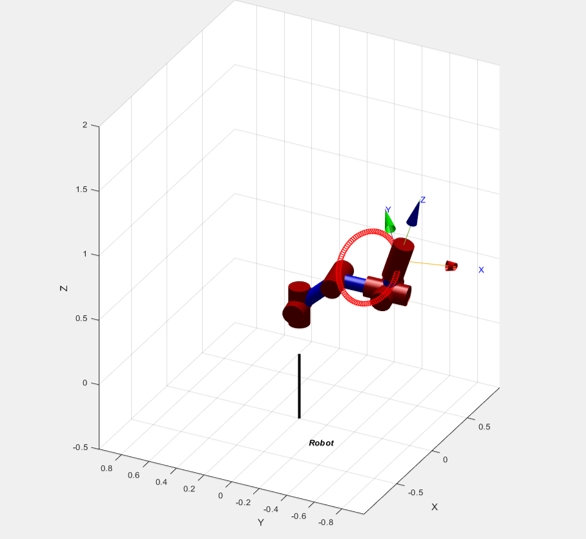
\includegraphics[width=0.6\textwidth]{Image/fig26.jpg}
    \caption{DrawCircle()函数末端圆形轨迹绘制效果}
    \label{fig:16}
\end{figure}
\subsubsection{空中截物检测}
\textbf{功能描述:}输入初始末端位姿T0;两个物体的初始位置P1、P2;初速度V1、V2;接物总时间$t_m$;中途接物后摇$t_s$;接到物体时规定末端位姿R1、R2(默认为$\left[\begin{matrix}0&0&1\\0&-1&0\\1&0&0\\\end{matrix}\right]$),输出机器人轨迹对应的旋转角解集组。

\textbf{原理分析}:设物体的初始位置为$P_{i0}$,初速度为$V_i$,加速度$A=\left[\begin{matrix}0\\-g\\0\\\end{matrix}\right]$。

于是$P=\int_{0}^{t}\left(V_i+A\tau\right)d\tau=P_{i0}+V_it+\frac{1}{2}At^2$,代入$ t$ 可得到任意时刻物体位置。

由于样条插值得到的轨迹为曲线,为减少计算量,仅考虑直线距离以规划接物顺序与时间。

代入$t_m$得到两物终点$P_{1m}$、$P2m$。机器人末端初始位置$P_0$已知。调整接中间物的时间$ t_c$使$\frac{\mid P\left(t_c\right)-P_0\mid}{\mid P_m-P\left(t_c\right)\mid}$ 最接近$\frac{t_c}{t_m-t_c}$ ,将此情况视为最优。更改先后顺序,选取两组最优轨迹总距离最小者。

\textbf{Code 3 {\quad} 空中截物检测函数}
\begin{lstlisting}
CatchBall(T0,P1,P2,V1,V2,tm,ts,R1,R2)
\end{lstlisting}

形式参数——T0:初始末端位姿 ;P1,P2:物体初始位置 ;
V1,V2:物体初速度; tm:接物限时 ;
ts:接物间隔  ;    R1,R2:接物时刻末端旋转矩阵。


\textbf{仿真展示}:如图\ref{fig:17}所示。左图为接到第一个物体时两物轨迹和机器人位姿,右图为接到第二个物体时两物轨迹(此时第一个物体的轨迹已停止继续生成)和机器人位姿。

\begin{figure}[htbp]
    \centering
    \subfigure[Situation 1]{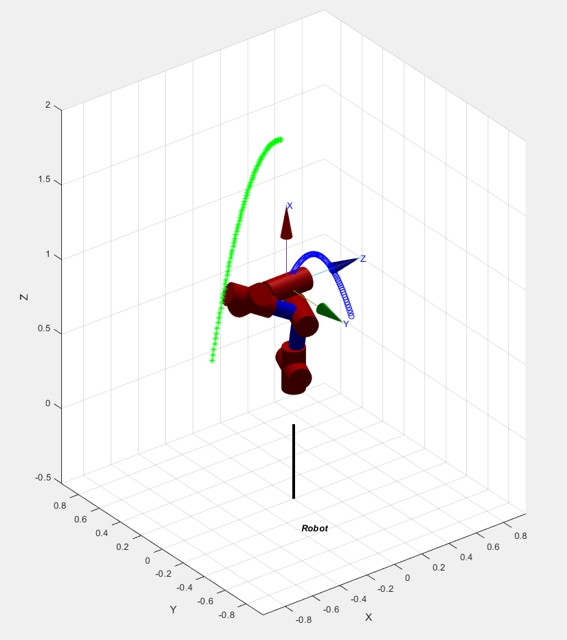
\includegraphics[width=0.4\textwidth]{Image/fig27.jpg}}
    \subfigure[Situation 2]{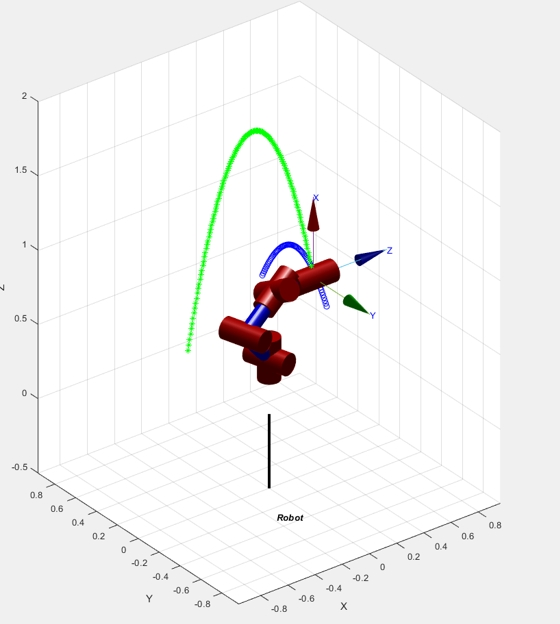
\includegraphics[width=0.4\textwidth]{Image/fig28.jpg}}
    \caption{空中截物检测仿真展示}
    \label{fig:17}
\end{figure}

如果我们是用\textbf{面向对象编程}的思想,我们可以将机器人的运动学功能封装成一个类MYROBOT,则可以通过我们写的这两个函数来实现机器人的运动学的特殊功能\verb|MYROBOT.DrawCircle();MYROBOT.CatchBall();|,用户并不需要了解具体的运动学原理,只需要调用这两个函数即可实现,这也很好的契合了我们一直以来所强调的工程思想。